% Version 2.x major modifications by: Vel (vel@latextemplates.com)

% ----- DOCUMENT CLASS LOADING ----- %

\documentclass[
12pt,                                            % The default document font size, options: 10pt, 11pt, 12pt
% oneside,                                       % Two side (alternating margins) for binding by default, uncomment to switch to one side
english,                                         % Thesis language, input ngerman for German for instance
singlespacing,                                   % Single line spacing, alternatives: onehalfspacing or doublespacing
liststotoc,                                      % Uncomment to add the list of figures/tables/etc to the table of contents
% toctotoc,                                      % Uncomment to add the main table of contents to the table of contents
% parskip,                                       % Uncomment to add space between paragraphs
headsepline,                                     % Uncomment to get a line under the header
% consistentlayout,                              % Uncomment to change the layout of the declaration, abstract and acknowledgements pages to match the default layout
]{main_class}                         % The class file specifying the document structure

% ----- DOCUMENT CONFIGURATIONS ----- %

% LaTeX doesnt like \include before parsing
% \begin{document} so we use \input here
% ----- Defining Colors Used in the Document ----- %

% ----- Color and macro for concepts ----- %
\definecolor{concept}{RGB}{255, 121, 36}
\newcommand{\concept}[1]{\textcolor{concept}{#1}}

% ----- Colors used in diagrams ----- %
\definecolor{wpblue}{RGB}{0, 0, 245}
\definecolor{wpred}{RGB}{234, 51, 36}

% ----- Colors in Matplotlib's default cycle ----- %
\definecolor{mplorange}{RGB}{238, 134, 54}
\definecolor{mplblue}{RGB}{59, 117, 175}
\definecolor{mplgreen}{RGB}{54, 151, 37}
\definecolor{mplred}{RGB}{197, 58, 50}
\definecolor{mplpurple}{RGB}{143, 108, 185}

% ----- Colors in Matplotlib's named cycle ----- %
\definecolor{mplb}{RGB}{0, 0, 245}
\definecolor{mplr}{RGB}{234, 54, 38}

% ----- Very custom colors used in the rematching plots ----- %
\definecolor{skyblue}{HTML}{204A87}
\definecolor{scarletred}{HTML}{A40000}
\definecolor{butter}{HTML}{C4A000}
\definecolor{highlightorange}{RGB}{247, 204, 121}

% ----- Colors used for the quotation admonition ----- %
\definecolor{DarkBluishGrey}{RGB}{0.325, 0.325, 0.349}                       % Define specific colors
%----------------------------------------------------------------------------------------
%	VARIOUS USED PACKAGES
%----------------------------------------------------------------------------------------

% ----- Classic Things ----- %
\usepackage[utf8]{inputenc}                      % required for inputting international characters
\usepackage[T1]{fontenc}                         % output font encoding for international characters
\usepackage{lmodern}
\usepackage[autostyle=true]{csquotes}            % required to generate language-dependent quotes in the bibliography


% ----- Maths Related ----- %
\usepackage{amsmath, amsfonts, amssymb}          % all the good math stuff
\usepackage{siunitx}                             % good macros for SI units


% ----- Figures Related ----- %
\usepackage{tikz}                                % create and include Tikz figures
\usetikzlibrary{matrix}
\usepackage{caption}                             % this and below are used for the
\usepackage{subcaption}                          % subfigures throughout the document


% ----- Tables Related ----- %
\usepackage{tabularray}                          % holy grail of tables
\UseTblrLibrary{amsmath}                         % Makes tabularray load amsmath and register better environments


% ----- Document Formating Related ----- %
\usepackage{titlesec}                            % to style chapter titles
\usepackage{awesomebox}                          % awesome boxes, includes fontawesome
\usepackage{appendix}                            % to make appendix appear properly in the table of content
\usepackage{xurl}                                % urls can break anywhere
\usepackage[
    bibstyle=numeric,
    citestyle=numeric-comp,
    sorting=none
]{biblatex}                                      % citations and bibliography
\usepackage{orcidlink}                           % include hyperlink patch to people's ORCID page | load after hyperref
\usepackage{microtype}                           % improves kerning, only include in last stages of compilation, takes time!

% Acronyms ------------------
\usepackage[
    acronym,                                     % add acronym type
    toc,                                         % add to toc
    section=section,                             % sections (glossary, acronyms) are actually sections
    nonumberlist,                                % remove backref numbers
]{glossaries}
\newcommand{\symboltype}{symbolslist}
\newglossary[slg]{symbolslist}{syi}{syg}{Symbols}% create symbolslist

% ----- References, Cross-Linking and Links Related ----- %
\usepackage{hyperref}                            % hyperlinks through the document | load before cleveref
\usepackage[capitalise, nameinlink]{cleveref}    % get smart references across the document | load last

% ----- Fonts Related ----- %
% \usepackage{utopia}                              % Use the Palatino font
% \usepackage{newtxtext,newtxmath}                 % Use the TeX Gyre Termes font
\usepackage{tgheros}                             % Use the TeX Gyre Heros font

                     % Load all necessary packages
% ----- Combined Entries ----- %
% Argument order: id, acronym, acronym written out, description
% Create both acronym and glossary entry with linking:
\newcommand{\newglossaryacronym}[4]{
    \newacronym{#1acr}{#2}{\acrlong{#1}}
    \newglossaryentry{#1}{
        name={#2 (#3)},
        text={#2},
        % symbol={#2},
        short={#2},
        long={#3},
        first={#3 (#2)},
        firstplural={#3\glspluralsuffix~(#2\glspluralsuffix)},
        description={#4\glsadd{#1acr}}
    }
}

% ----- Nomenclature ----- %

\newglossaryentry{detail}{
    name={detail},
    text={detail},
    description={Additional info}}

\newglossaryentry{atomic-mass}{
    name={atomic-mass},
    text={atomic-mass},
    description={Mass of an atom}}

% ----- Detailed Acronyms, they show up in the nomenclature ----- %

\newglossaryacronym{SRT}{SRT}{Special Relativity Theory}{
    Special Relativity Theory
}

% ----- Acronyms ----- %

\newacronym{}{}{}

% ----- Symbols ----- %

\newglossaryentry{M}{
    type=\symboltype,
    sort={M},
    name={\(\mathbf{ M }\)},
    text={Mass},
    symbol={\(M\)},
    description={Mass. Unit: \unit{\kilogram}}
}

\glsenableentrycount                             % Enable ref counting when displaying, adds some compile time to the document
             % Definitions for the glossary
%----------------------------------------------------------------------------------------
%	SIUNITX SETTINGS
%----------------------------------------------------------------------------------------

\sisetup{
    exponent-product=\times,      % operator between number and 10^n
    print-unity-mantissa=false,  % no 1 x 10^3, only 10^3
    % inter-unit-product=\cdot,
    % separate-uncertainty,
    % table-align-uncertainty,
}
\DeclareSIUnit \barn{b}                    % As barn was remove we need to define it

\DeclareSIPower \nth\tothenth{n}           % Used for arbitrary powers of n
\DeclareSIPower \pernth\totheminusnth{-n}  % Used for arbitrary inverse powers of n                      % Custom siunitx settings
% ----- MARGIN SETTINGS ----- %

\geometry{
	paper=a4paper, % Change to letterpaper for US letter
	inner=2.5cm, % Inner margin
	outer=2.5cm, % Outer margin
	bindingoffset=.5cm, % Binding offset
	top=1.5cm, % Top margin
	bottom=1.5cm, % Bottom margin
	% showframe, % Uncomment to show how the type block is set on the page
}                     % Document geometry settings
% ----- Defining Custom AWESOMEBLOCKs for use in the Document ----- %

% Quotation block
\newenvironment{quoteblock}{
    \begin{awesomeblock}[DarkBluishGrey]{2pt}{\Large \faQuoteLeft\;{\color{lightgray}\faQuoteRight}}{DarkBluishGrey}
    }{
    \end{awesomeblock}
}                  % Custom blocks for awesomeblocks
%----------------------------------------------------------------------------------------
%	ARTICLE INFORMATION
%----------------------------------------------------------------------------------------

\thesistitle{Title} % Print with \ttitle

\supervisor{Prof. Name} % Print with \supname

\examiner{} % Print with \examname

\degree{Doctor of Philosophy} % Print with \degreename

\author{Name \textsc{Surname}} % Print with \authorname

\addresses{} % Print with \addressname

\subject{Philosophy} % Print with \subjectname

\keywords{} % Print with \keywordnames

\university{ref} % Print with \univname

\department{ref} % Print with \deptname

\group{ref} % Print with \groupname

\faculty{ref}{Org_name} % Print with \facname                  % Thesis information for document class
% ----- Page thumbs to the side ----- %
\usepackage{scrlayer-scrpage}                    % allows setting layers on pages (e.g. chapterthumbs/headers/footers)

% \KOMAoptions{numbers=noenddot}

% Chapterthumbs
% Adapted by jdilly to use tikz according to 
% https://tex.stackexchange.com/questions/526904/scrreprt-thumb-indices-with-scrlayer-scrpage-use-any-shape-as-chapterthumb
% needs, tikz, scrlayer-scrpage, koma, 
% original example in https://komascript.de/komascriptbuch7examples 
\newlength{\chapterthumbwidth}
\newlength{\chapterthumbheight}

\newcommand*{\firstchapterthumbskip}{.065\paperheight}
\newcommand*{\lastchapterthumbskip}{\firstchapterthumbskip}
\setlength{\chapterthumbheight}{3.5em}
\setlength{\chapterthumbwidth}{.055\paperwidth}
\newcommand*{\chapterthumbskip}{.065\paperheight}
\colorlet{chapterthumbboxcolor}{black}
\newcommand*{\chapterthumbcolor}{white}
% \newcommand*{\chapterthumbformat}{\@chapapp~\thechapter}
\newcommand*{\chapterthumbformat}{\thechapter}
\newkomafont{chapterthumb}{\normalfont\Large\color{\chapterthumbcolor}}

\usetikzlibrary{shapes.misc, positioning}

\makeatletter
% TIKZ Style
\newcommand*\chapterthumb@box{%
  \usekomafont{chapterthumb}%
    \parbox[c][\chapterthumbheight][c]{\chapterthumbwidth}{%
      \centering
      \begin{tikzpicture} 
        % second rectangle to hide rounded corner on page border
        \ifodd\value{page}
            \node[rectangle, 
                fill=chapterthumbboxcolor,
                minimum width=0.9\chapterthumbwidth, 
                minimum height=\chapterthumbheight,
                ] at (0.1,0){};
        \else
            \node[rectangle, 
                fill=chapterthumbboxcolor,
                minimum width=0.9\chapterthumbwidth, 
                minimum height=\chapterthumbheight,
                ] at (-0.1,0){};
        \fi
        % rectangle with content
        \node[rectangle, 
              fill=chapterthumbboxcolor,
              minimum width=\chapterthumbwidth, 
              minimum height=\chapterthumbheight,
              rounded corners=2pt,
              ] at (0,0){\chapterthumbformat};
      \end{tikzpicture}%
    }%
}

% Original style
% \newcommand*\chapterthumb@box{%
%             \rotatebox[origin=tl]{90}{%
%               \setlength{\fboxsep}{0pt}%
%               \colorbox{chapterthumbboxcolor}{%
%                 \parbox[c][\chapterthumbheight][c]%
%                 {\chapterthumbwidth}{%
%                   \centering
%                   \color{\chapterthumbcolor}%
%                   \usekomafont{chapterthumb}{%
%                     \chapterthumbformat
%                   }}}}%
% }

\newcommand*{\chapterthumbbox}{%
    \if@mainmatter
    \ifnum\value{chapter}>\z@
    \ifnum \value{chapterthumb}<\z@
    \else
    \begingroup
    \protected@edef\reserved@a{\chapterthumbformat}%
    \ifx\reserved@a\lastchapterthumbformat\else
    \stepcounter{chapterthumb}%
    \global\let\lastchapterthumbformat\reserved@a
    \fi
    \@tempcnta=\numexpr
    \dimexpr
    \paperheight
    -\firstchapterthumbskip
    -\chapterthumbwidth
    -\lastchapterthumbskip
    \relax / \dimexpr
    \chapterthumbskip
    \relax
    +1
    \relax
    \ifnum \value{chapterthumb}<\@tempcnta
    \else
    \setcounter{chapterthumb}{0}%
    \fi
    \vspace*{%
        \dimexpr
        \firstchapterthumbskip
        + ( \chapterthumbskip )
        * \value{chapterthumb}%
        - \baselineskip
        \relax
    }\par
    \setlength{\fboxsep}{0pt}%
    \ifodd\value{page}
    \hfill
    \makebox[0pt][r]{\chapterthumb@box}%
    \else
    \makebox[0pt][l]{\chapterthumb@box}%
    \fi
    \endgroup
    \fi
    \fi
    \fi
}
\makeatother

\newcounter{chapterthumb}
\setcounter{chapterthumb}{10000}
\newcommand*{\lastchapterthumbformat}{\relax}

\DeclareNewLayer[%
background,%
outermargin,%
% oddpage,%
% rightmargin,%
contents=\chapterthumbbox
]{chapterthumb}

\newcommand*\EnableChapterthumb{%
    \IfLayerAtPageStyle{scrheadings}{chapterthumb}{}
    {\AddLayersToPageStyle{@everystyle@}{chapterthumb}}%
}
\newcommand*\DisableChapterthumb{%
    \RemoveLayersFromPageStyle{@everystyle@}{chapterthumb}%
}
                 % All the magic for page thumbs to the side
% ----- Hyperref setup for frontmatter ----- %
\hypersetup{
    pdfpagemode={UseOutlines},
    bookmarksopen=true,
    bookmarksopenlevel=0,
    hypertexnames=false,
    colorlinks=true,                             % Set to false to disable coloring links
    citecolor=black,                           % The color of citations
    linkcolor=red,                               % The color of references to document elements (sections, figures, etc)
    linktoc=all,                                 % Includes page-numbers in links
    urlcolor=mdtRed,                             % The color of hyperlinks (URLs)
    pdfstartview={FitV},
    unicode,
    breaklinks=true,
}         % Update hyperref setup for titlepage

\setcounter{secnumdepth}{3}                      % Detailing level of section numbering in table of content
\addbibresource{Bibliography.bib}                % Load the bibliography definitions file
\bibliographystyle{plain}
\makenoidxglossaries                             % Prepare the glossary entries (does not display yet)

% ----- FRONTMATTER ----- %

\begin{document}

\frontmatter                                     % Roman page numbering style (i, ii, iii, iv...) for the pre-content pages
\pagestyle{plain}                                % Default to the plain heading style

\begin{titlepage}
\begin{center}

\vspace*{.06\textheight}
\vspace{1cm}
{\scshape\LARGE \univname\par} % University name
\vspace{0.8cm}

\begin{figure}[ht]
    \centering
    \includegraphics[width=\textwidth]{Figures/Logos/UoLlogo.eps}
\end{figure}

\HRule \\[0.4cm] % Horizontal line
{\huge \bfseries \ttitle\par}\vspace{0.4cm} % Thesis title
\HRule \\[1cm] % Horizontal line

\vspace{1cm}

\begin{minipage}[t]{0.4\textwidth}
\begin{flushleft} \large
\text{Submitted by:}\\
\href{https://orcid.org/my-orcid?orcid=0000-0001-8012-1440}{\authorname} % Author name - remove the \href bracket to remove the link
\end{flushleft}
\end{minipage}
\begin{minipage}[t]{0.4\textwidth}
\begin{flushright} \large
\text{Supervised by:}\\
\href{https://www.researchgate.net/profile/Tobias-Persson}{Dr. Tobias~\textsc{Persson}}\\
\href{https://orcid.org/0000-0002-9857-1703}{Dr. Rogelio~\textsc{Tomás}}\\
\href{https://orcid.org/0000-0002-5410-7706}{Dr. Oznur~\textsc{Apsimon}}\\
\href{https://orcid.org/0000-0001-7085-0973}{\supname}\\
\end{flushright}
\end{minipage}

\vspace{1.5cm}

\vfill

\large {Thesis submitted in accordance with the requirements of the\\}
\univname, \deptname \\
\large {for the degree of Doctor in Philosophy}

\vfill

{\large \today}\\[4.5cm] % Date

\vfill
\end{center}
\end{titlepage}              % Generate the title page
% ----- Commands for recurrent expressions ----- %

% Command for asterisks
\newcommand{\asterisk}{\(^{\ast}\) }  % needs the trailing space


% ----- Commands for recurrent expressions in math mode ----- %

% Command for the absolute value of something
\newcommand{\abs}[1]{\left\lvert #1 \right\rvert}

% Command for the complex conjugate of something
\newcommand{\conj}[1]{#1^{\ast}}
               % Custom commands for math elements
%-----------------------------%
%	     USER COMMANDS        %
%-----------------------------%

% Mark some text as todo, in red
\newcommand{\todo}[1]{\textcolor{red}{TODO: #1}}

% Used for listing of code developments
\newcommand{\ilparagraph}[2]{\paragraph{\textbf{#1}~{#2}\textbf{.}}}               % Miscellanea custom commands
% ----- Hyperref setup for mainmatter ----- %
\hypersetup{
    bookmarksopen=true,
    bookmarksopenlevel=0,
    hypertexnames=false,
    citecolor=cern,                              % The color of citations
    linkcolor=cern,                              % The color of references to document elements (sections, figures, etc)
    linktoc=all,                                 % includes page-numbers in links
    urlcolor=mdtRed,                             % The color of hyperlinks (URLs)
    unicode,
    breaklinks=true,
    hypertexnames=false,                         % Fixes wrong linking with subequations, but might have side-effects (check index links!)
}     % Update hyperref setup for fronmatter

\begin{declaration}

\vspace{1cm}

The authors declare that they have no known competing financial interests or personal relationships that could have appeared to influence the work reported in this paper.

\end{declaration}

\cleardoublepage
\begin{abstract}

The abstract here.

\end{abstract}

\glsresetall                                     % reset glossary entries counts for the next chapter

\begin{acknowledgements}
% \addchaptertocentry{\acknowledgementname} % Add the acknowledgements to the table of contents
\vspace{0.8cm}

The acknowledgements here.

\end{acknowledgements}
\newpage
\vspace*{0.4\textheight}
\begin{center}
	\noindent\enquote{\itshape Everything always breaks...}\bigbreak
	Do not break rules!
\end{center}

\setcounter{tocdepth}{1}                         % How detailed table of content should be
\tableofcontents                                 % Prints the main table of contents
% Output ----------------------------------------------------------------------------------------------------
% for different styles see: https://www.dickimaw-books.com/gallery/glossaries-styles/

\addchap{Glossary}
\glsnogroupskiptrue
% \glsaddall                                       % for testing only, remove at some point
\setacronymstyle{long-short}                     % First use displays the long form, subsequent uses display the short form
\let\Oldglsnamefont\glsnamefont
\renewcommand{\glsnamefont}[1]{\makefirstuc{#1}} % capitalize first letter in each entry
\printnoidxglossary[title=Nomenclature]          % print the nomenclature glossary

\let\glsnamefont\Oldglsnamefont                  % undo first letter capitalization rule
\printnoidxglossary[type=\acronymtype]           % print the acronyms glossary
\printnoidxglossary[type=\symboltype]            % print the symbols glossary

\glsresetall                                     % reset glossary entries counts after displaying glossary
               % Will now display the glossary
% ----- Hyperref setup for list of figures and list of tables ----- %
\hypersetup{
    bookmarksopen=true,
    bookmarksopenlevel=0,
    hypertexnames=false,
    colorlinks=black,                            % DO NOT COLOR LINKS IN LIST OF FIGURES AND LIST OF TABLES - This way the 
    citecolor=black,                              % The color of citations
    linkcolor=black,                             % The color of references to document elements (sections, figures, etc)
    linktoc=all,                                 % includes page-numbers in links
    unicode,
    breaklinks=true,
    hypertexnames=false,                         % Fixes wrong linking with subequations, but might have side-effects (check index links!)
}        % Update hyperref setup for list of figures and list of tables
\listoffigures                                   % Prints the list of figures
\listoftables                                    % Prints the list of tables

% ----- CHAPTERS ----- %

\mainmatter                                      % Numeric (1,2,3...) page numbering
% ----- Hyperref setup for mainmatter ----- %
\hypersetup{
    pdfpagemode={UseOutlines},
    bookmarksopen=true,
    bookmarksopenlevel=0,
    hypertexnames=false,
    colorlinks=true,                             % Set to false to disable coloring links
    citecolor=black,                              % The color of citations
    linkcolor=black,                              % The color of references to document elements (sections, figures, etc)
    linktoc=all,                                 % includes page-numbers in links
    urlcolor=black,                               % The color of hyperlinks (URLs)
    pdfstartview={FitV},
    unicode,
    breaklinks=true,
    hypertexnames=false,                         % Fixes wrong linking with subequations, but might have side-effects (check index links!)
}      % Update hyperref setup for mainmatter
\pagestyle{thesis}                               % Return the page headers back to the "thesis" style

\EnableChapterthumb                              % Start displaying chapterthumbs in the mainmatter

%----------------------------------------------------------------------------------------
%	REDEFINE CHAPTER TITLE STYLE
%----------------------------------------------------------------------------------------

% See doc of titlesec page 22 (https://mirror2.sandyriver.net/pub/ctan/macros/latex/contrib/titlesec/titlesec.pdf)
% TODO: fix the slight antisymmetry in vspace bellow CHAPTER N

\titleformat{\chapter}[display]
{\Large\filcenter}
{\titlerule[1pt]%
\vspace{1pt}%
\titlerule
\vspace{1pc}%
\LARGE\MakeUppercase{\chaptertitlename} \thechapter}{1pc}
{\titlerule
\vspace{1pt}%
\titlerule[1pt]%
\vspace{1pc}%
\Huge}               % Custom chapter style for the mainmatter
\chapter{Theory}
\label{chapter:theory}

Theory is described in \gls{detail}.
For a complete understanding of the \acrshort{SRT}, one is referred to~\cite{ADP:Einstein:On_The_Electrodynamics_Of_Moving_Bodies}.

%----------------------------------------------------------------------------------------

\section{Theory: section1}
\label{section:section1}

This section stands for the theory clarification.

\subsection{Theory: subsection1}
\label{subsection:subsection1}

This subsection stands for the theory section clarification.
The formula describing the variable \(X_{Y}\) is given by the equation:

\begin{equation}
    X_Y = X + Y \text{ ,}
    \label{equation:XY_equation}
\end{equation}
where \(X\) is the variable and \(Y\) is the variable too.

\begin{align}
    X_Y =
    \tikz[baseline]{
        \node[draw=red,rounded corners,anchor=base] (m1)
        {\(\displaystyle X\)};
        \node[below of=m1] (l1) {Variable X};
        \draw[-,red] (l1) -- (m1);
    }
    +
    \tikz[baseline]{
        \node[draw=red,rounded corners,anchor=base] (m2)
        {\(\displaystyle Y\)};
        \node[below of=m2] (l2) {Variable Y};
        \draw[-,red] (l2) -- (m2);
    }
    + \ldots
    \label{equation:XY_sum}
\end{align}

Moving on to figures.
\Cref{figure:atom} illustrates the well-know \concept{atomic structure} with an \gls{atomic-mass} \glssymbol{M}.

\begin{figure}[!htb]
    \centering
    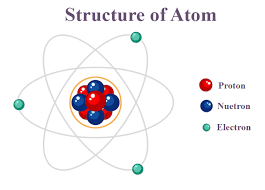
\includegraphics[width=0.9\linewidth]{Figures/Theory/atom.png}
    \caption{Atomic structure.}
    \label{figure:atom}
\end{figure}

Next two graphs show the examples of molecules.

\begin{figure}[!hbt]
    \centering
    \begin{subfigure}[b]{0.495\textwidth}
        \centering
        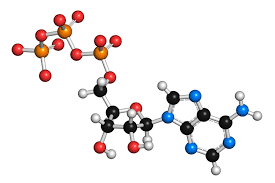
\includegraphics[width=\textwidth]{Figures/Theory/molecules.png}
        \caption{Molecules 1.}
        \label{fig:molecules1}
    \end{subfigure}
    \hfill
    \begin{subfigure}[b]{0.485\textwidth}
        \centering
        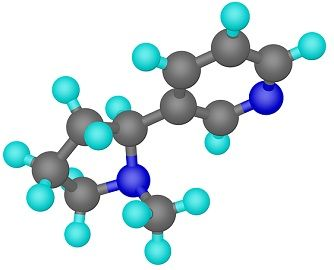
\includegraphics[width=\textwidth]{Figures/Theory/molecules1.jpg}
        \caption{Molecules 2.}
        \label{fig:molecules2}
    \end{subfigure}
    \caption{Molecules.}
    \label{fig:molecules}
\end{figure}

\subsection{Theory: subsection2}
\label{subsection:subsection2}

\begin{noteblock}
    Keeping forward.
\end{noteblock}

There were several atomic structure concepts.

Some concepts are presented in \cref{table:concepts}.
\begin{table}[!hbt]
    \centering
    \begin{tblr}{colspec={ccc}}
        \hline
        \SetCell[r=2,c=1]{m,c} Model & \SetCell[c=2]{c} Author       \\
        \cline{2,3}
                    &  Author      \\
        \hline
        Model1      &   G. Thomson    \\
        Model2      &  E. Rezerford  \\
        Model3      &   N. Bohr  \\
        Model4      &   Quantum mechanics society  \\
        \hline
    \end{tblr}
    \caption{Atomic structure models.}
    \label{table:concepts}
\end{table}

\glsresetall                                     % reset glossary entries counts for the next chapter


% ----- APPENDICES ----- %

\appendix                                        % Declare following "chapters" are Appendices

\chapter{Appendix Title Here}
\label{appendix:template}

Write your Appendix content here.

\DisableChapterthumb                             % So we don't get chapterthumbs in the bibliography

% ----- BIBLIOGRAPHY ----- %

\addcontentsline{toc}{chapter}{Bibliography}
\printbibliography

\end{document}